%
% latex-sample.tex
%
% This LaTeX source file provides a template for a typical research paper.
%

%
% Use the standard article template.
%
\documentclass[twocolumn]{article}
\usepackage{float}
\usepackage{graphicx}

\begin{document}
	
\section{Performances optimization and input parameter analysis}

The work-stealing scheduler module takes as input three different execution parameters: 
	\begin{itemize}
		\item Array size; 
		\item Number of servers that must be created by the scheduler;
		\item The sequential cut-off parameter that is the size of array that will be processed sequentially even in multi-threading execution of the scheduler. 
	\end{itemize}

All these parameters affects the concurrent ordering execution time, and relative speed-up on the sequential one. To estimate the 
\begin{figure}[h!]
		\centering
		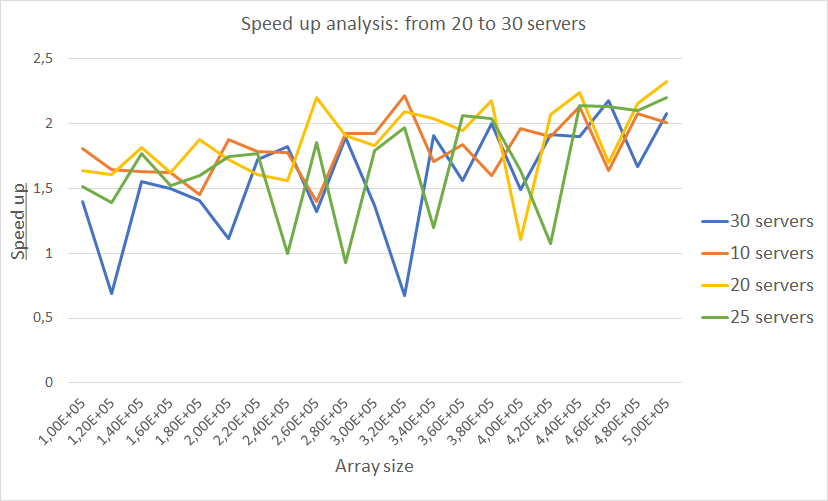
\includegraphics[width=1.0\linewidth]{imgs/SpeedUP5-20server}
		\caption{}
		\label{fig:speedup5-20server}
\end{figure}
\section{Prova}


\begin{figure}[h!]
	\centering
	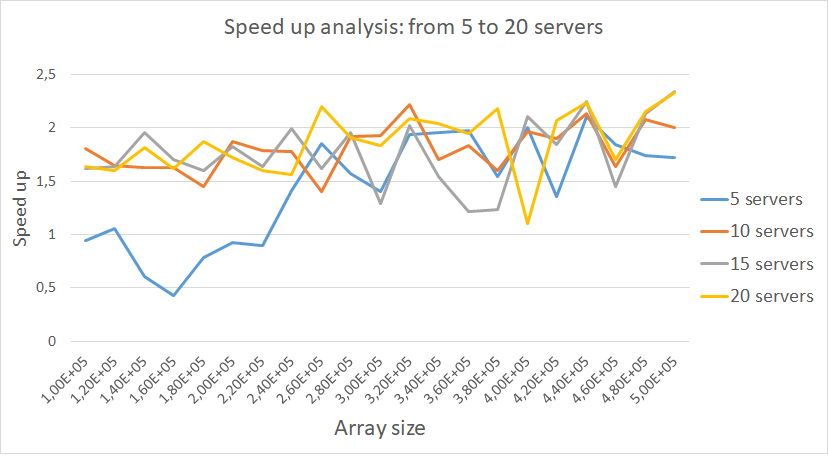
\includegraphics[width=1.0\linewidth]{imgs/SpeedUp20-30servers}
	\caption{}
	\label{fig:speedup20-30servers}
\end{figure}

\begin{figure}[h!]
	\centering
	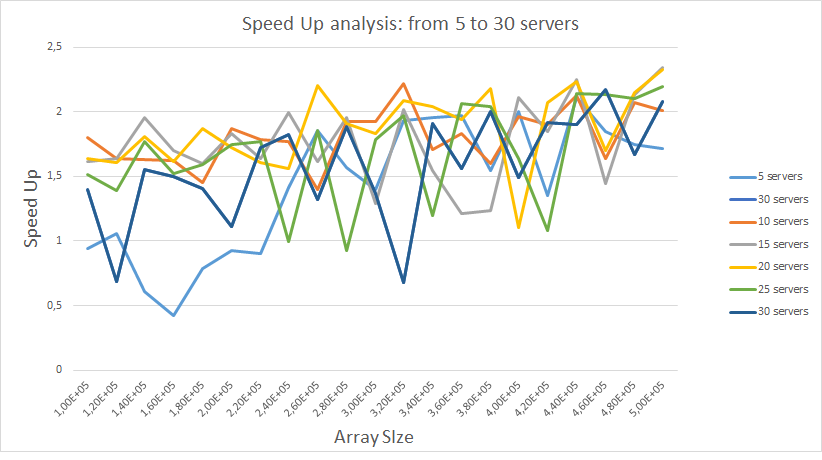
\includegraphics[width=1.0\linewidth]{imgs/SpeedUp5-30servers}
	\caption{}
	\label{fig:speedup5-30servers}
\end{figure}

\begin{figure}[h]
	\centering
	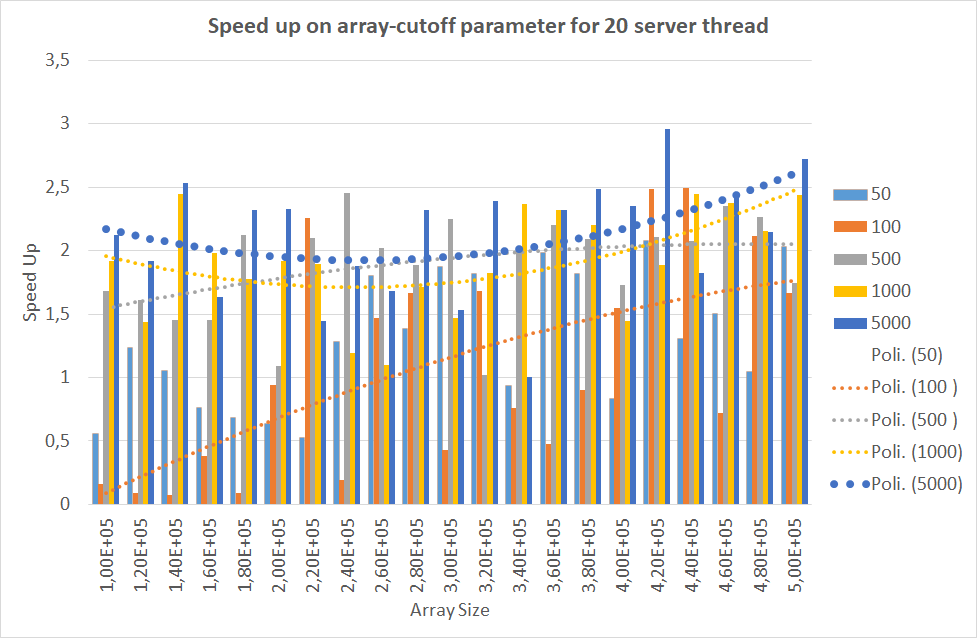
\includegraphics[width=1.0\linewidth]{imgs/SpeedUp20ServerArrayAndCutOffAnalysis}
	\caption{}
	\label{fig:speedup20serverarrayandcutoffanalysis}
\end{figure}
\begin{figure}[h!]
	\centering
	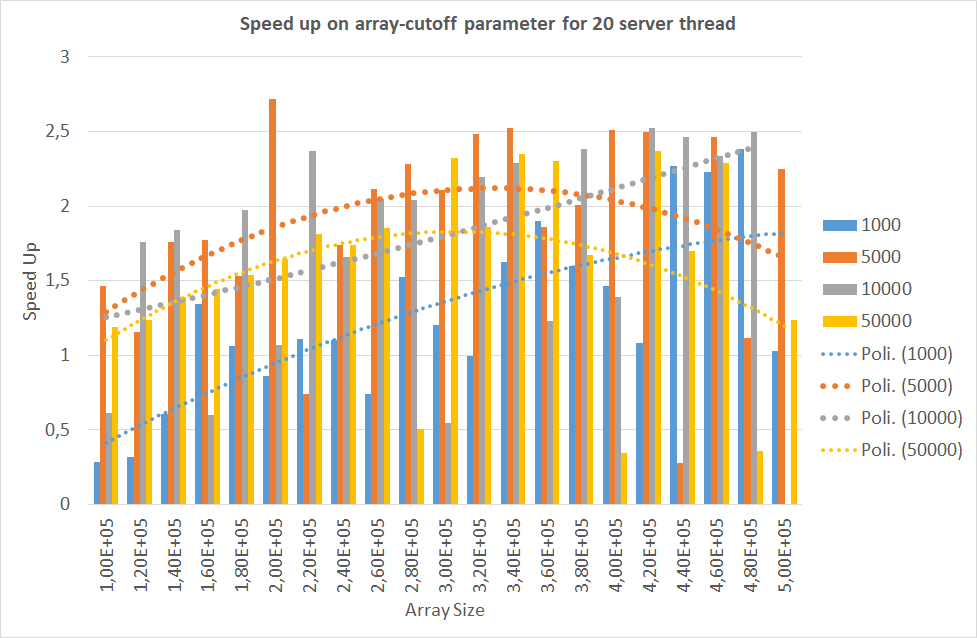
\includegraphics[width=1.0\linewidth]{imgs/SpeedUp20ServerHigherCutoffValuesAnalysis}
	\caption{}
	\label{fig:speedup20serverhighercutoffvaluesanalysis}
\end{figure}

\begin{figure}[h!]
	\centering
	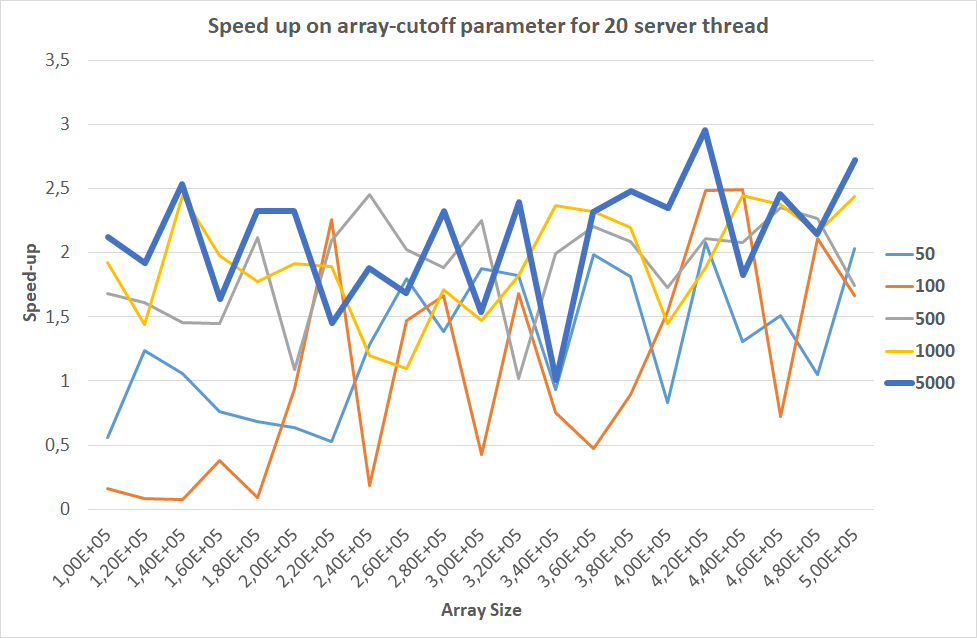
\includegraphics[width=1.0\linewidth]{imgs/SpeedUpAnalysis20ServersArrayAndCutOffAnalysisLINESGraph}
	\caption{}
	\label{fig:speedupanalysis20serversarrayandcutoffanalysislinesgraph}
\end{figure}

\begin{figure}[h!]
	\centering
	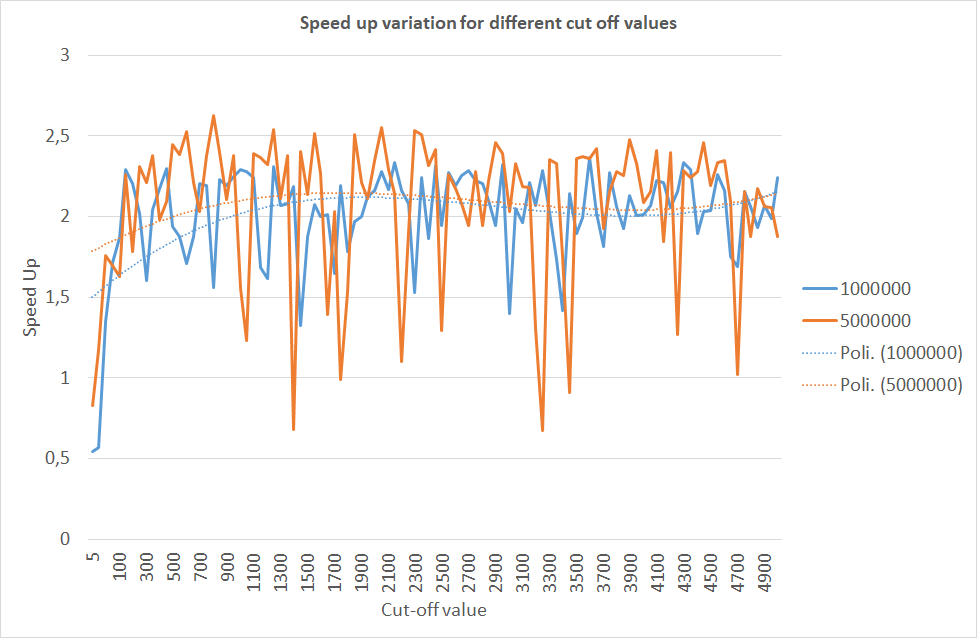
\includegraphics[width=1.0\linewidth]{imgs/SpeedUpForDifferentCutOff100-500mila}
	\caption{}
	\label{fig:speedupfordifferentcutoff100-500mila}
	
\end{figure}

	
	

	
\end{document}
